\documentclass[11pt,a4paper]{report}

\usepackage[utf8]{inputenc}
\usepackage[T1]{fontenc}
\usepackage[margin=2cm, headheight=15pt]{geometry}
\usepackage{graphicx}
\usepackage{xcolor}
\usepackage{amsmath,amssymb}
\usepackage{booktabs}
\usepackage{array}
\usepackage{listings}
\usepackage{hyperref}
\usepackage{fancyhdr}
\usepackage{titlesec}

% Palette de couleurs professionnelle INPT
\definecolor{inptblue}{HTML}{1E40AF}
\definecolor{inptdark}{HTML}{0F172A}
\definecolor{inptlight}{HTML}{EFF6FF}
\definecolor{codebg}{HTML}{F8FAFC}
\definecolor{codeframe}{HTML}{CBD5E1}
\definecolor{codekw}{HTML}{1D4ED8}
\definecolor{codestr}{HTML}{15803D}
\definecolor{codecmt}{HTML}{64748B}
\definecolor{slate}{HTML}{334155}
\definecolor{alertred}{HTML}{DC2626}
\definecolor{validgreen}{HTML}{16A34A}
\definecolor{goldstreak}{HTML}{D97706}

\hypersetup{
    colorlinks=true,
    linkcolor=inptblue,
    urlcolor=inptblue,
    pdftitle={Manuel Integral d'Apprentissage et Revue de Code - IPv4 Subnet Toolkit v1.2.0},
    pdfauthor={INPT - Cursus Ingenieur ASEDS}
}

\pagestyle{fancy}
\fancyhf{}
\fancyhead[L]{\small\textbf{\textcolor{inptblue}{IPv4 Subnet Toolkit v1.2.0}} --- Manuel d'Apprentissage}
\fancyhead[R]{\small\textcolor{slate}{INPT ASEDS --- Python / PyQt6}}
\fancyfoot[C]{\thepage}

\setlength{\parskip}{0.5em}
\setlength{\parindent}{0pt}

% Configuration des listings de code
\lstset{
    backgroundcolor=\color{codebg},
    frame=single,
    rulecolor=\color{codeframe},
    basicstyle=\ttfamily\footnotesize,
    keywordstyle=\color{codekw}\bfseries,
    stringstyle=\color{codestr},
    commentstyle=\color{codecmt}\itshape,
    breaklines=true,
    showstringspaces=false,
    tabsize=4,
    captionpos=b,
    literate=
        {é}{{\'e}}1
        {è}{{\`e}}1
        {ê}{{\^e}}1
        {ë}{{\"e}}1
        {à}{{\`a}}1
        {ù}{{\`u}}1
        {û}{{\^u}}1
        {ô}{{\^o}}1
        {î}{{\^i}}1
        {ï}{{\"i}}1
        {ç}{{\c{c}}}1
        {É}{{\'E}}1
        {À}{{\`A}}1
        {→}{{$\rightarrow$}}1
        {≥}{{$\ge$}}1
        {≤}{{$\le$}}1
        {−}{{$-$}}1
        {✓}{{$\checkmark$}}1
        {✕}{{$\times$}}1
        {•}{{$\bullet$}}1
        {…}{{\dots}}1
}

\newcommand{\techbox}[2]{%
    \vspace{0.4em}
    \noindent\fcolorbox{inptblue}{inptlight}{%
        \parbox{\dimexpr\linewidth-2\fboxsep-2\fboxrule\relax}{%
            \textbf{\textcolor{inptblue}{#1}}\\[0.3em]
            #2
        }%
    }%
    \vspace{0.4em}
}

\newcommand{\alertbox}[2]{%
    \vspace{0.4em}
    \noindent\fcolorbox{alertred}{codebg}{%
        \parbox{\dimexpr\linewidth-2\fboxsep-2\fboxrule\relax}{%
            \textbf{\textcolor{alertred}{#1}}\\[0.3em]
            #2
        }%
    }%
    \vspace{0.4em}
}

\newcommand{\successbox}[2]{%
    \vspace{0.4em}
    \noindent\fcolorbox{validgreen}{codebg}{%
        \parbox{\dimexpr\linewidth-2\fboxsep-2\fboxrule\relax}{%
            \textbf{\textcolor{validgreen}{#1}}\\[0.3em]
            #2
        }%
    }%
    \vspace{0.4em}
}

\begin{document}

% ============================================================================
% PAGE DE TITRE
% ============================================================================
\begin{titlepage}
    \centering
    \vspace*{1cm}
    {\Large \textbf{\textcolor{inptblue}{INSTITUT NATIONAL DES POSTES ET T\'EL\'ECOMMUNICATIONS (INPT)}}}\\[0.3cm]
    {\large Cursus Ing\'enieur --- Fili\`ere ASEDS (Syst\`emes Embarqu\'es \& R\'eseaux)}\\[1.8cm]

    \rule{\linewidth}{0.6mm}\\[0.5cm]
    {\Huge \textbf{\textcolor{inptblue}{IPv4 Subnet Toolkit v1.2.0}}}\\[0.4cm]
    {\LARGE \textbf{Manuel Int\'egral d'Apprentissage, Math\'ematiques R\'eseau,}}\\[0.2cm]
    {\LARGE \textbf{Architecture Logicielle \& Guide d'Ing\'enierie du Code Source}}\\[0.3cm]
    \rule{\linewidth}{0.6mm}\\[1cm]

    {\large \textit{Recueil exhaustif de la documentation p\'edagogique et technique : Alg\`ebre bool\'eenne 8/32 bits, d\'ecoupage VLSM d\'ecroissant, solveurs MTU / LPM / Checksum 16 bits, ing\'enierie d'interface PyQt6 anti-saturation, mod\`ele MVC d\'ecoupl\'e et blueprint de portage Java 17/21 OOP.}}\\[1.2cm]

    \begin{center}
        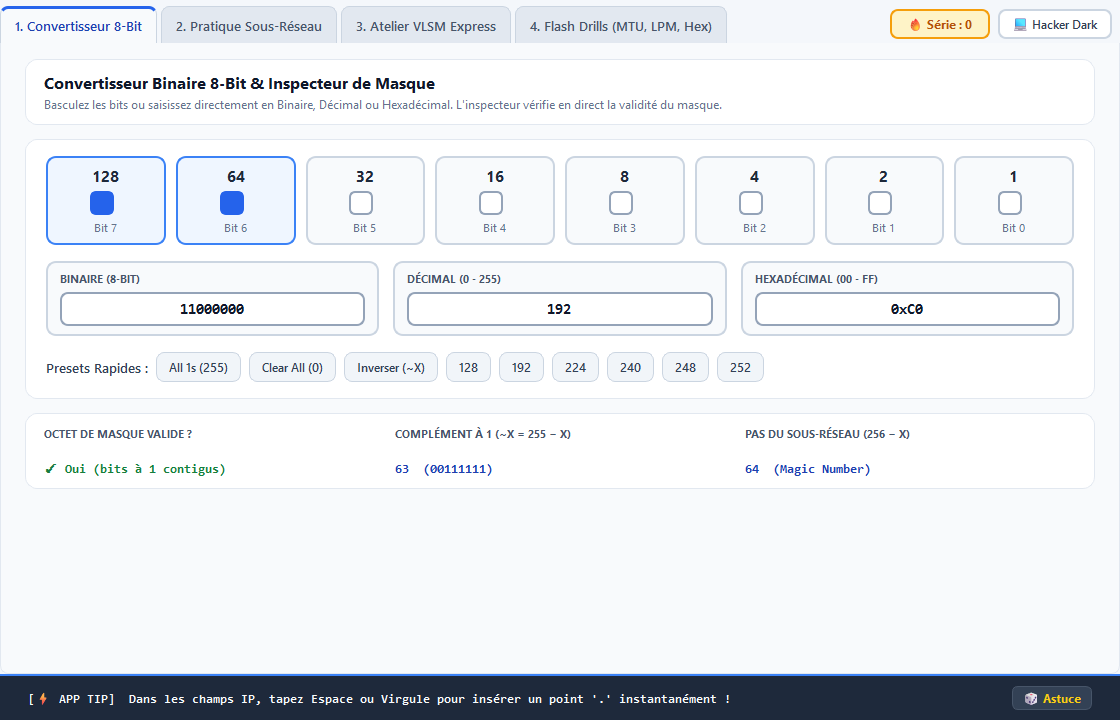
\includegraphics[width=0.88\textwidth]{../screenshots/01_tab1_mask_valid_light.png}
    \end{center}

    \vfill
    {\large \textbf{Version 1.2.0 --- Octobre 2026}}\\
    {\normalsize \'Edition Int\'egrale d\'edi\'ee aux \'Etudiants et Enseignants INPT ASEDS}
\end{titlepage}

\tableofcontents
\newpage

% ============================================================================
% PARTIE I : ARCHITECTURE FONDAMENTALE & MATHEMATIQUES RESEAU
% ============================================================================
\part{Architecture Fondamentale \& Math\'ematiques R\'eseau}

\chapter{Architecture Globale : Du Monolithe v1.0.0 \`a la Clean Architecture v1.2.0}

\section{Pourquoi Refactoriser en Deux Paquetages D\'ecoupl\'es ?}
Dans la version initiale \texttt{v1.0.0}, l'int\'egralit\'e du programme r\'esidait dans un fichier unique \texttt{converter.py} (1\,171 lignes de code). Les calculs d'adresses IP, l'algorithmique binaire et la validation des saisies \'etaient imbriqu\'es \`a l'int\'erieur des m\'ethodes de classes graphiques \texttt{QWidget}.

Pour la version \textbf{v1.2.0}, nous appliquons le principe fondamental de \textbf{S\'eparation des Pr\'eoccupations (\textit{Separation of Concerns --- SoC})} :
\begin{enumerate}
    \item \textbf{Z\'ero d\'ependance GUI dans \texttt{engine/}} : Aucun fichier du paquetage moteur n'importe \texttt{PyQt6}. Le moteur ne manipule que des types primitifs Python (\texttt{int}, \texttt{str}, \texttt{bool}, \texttt{list}) et des objets de transfert immuables (\texttt{@dataclass(frozen=True)}).
    \item \textbf{Testabilit\'e unitaire imm\'ediate} : 100\,\% des calculs, des exercices VLSM et des cas limites peuvent \^etre ex\'ecut\'es et valid\'es en ligne de commande en quelques millisecondes, sans devoir initialiser de serveur X ou de contexte graphique.
    \item \textbf{Portabilit\'e vers Java OOP (Cursus ASEDS)} : Chaque \texttt{@dataclass} correspond rigoureusement \`a un \texttt{record} Java 16+ ou \`a une classe POJO finale. Chaque classe de service (\texttt{IPv4MathEngine}, \texttt{VlsmSolver}, \texttt{DrillsSolver}) regroupe des m\'ethodes pures sans \'etat, triviales \`a traduire en m\'ethodes \texttt{public static} en Java.
\end{enumerate}

\newpage
\section{Sch\'ema du Mod\`ele MVC D\'ecoupl\'e}
\begin{center}
\begin{lstlisting}[basicstyle=\ttfamily\scriptsize]
                  +------------------------------+
                  |         converter.py         |
                  |   Point d'Entree & Boucle Qt |
                  +--------------+---------------+
                                 | Demarre
                                 v
                  +----------------------------------------------+
                  |              ui/main_window.py               |
                  |  Fenetre Racine, Menu, Themes & Mediateur    |
                  +------+-----------+-----------+---------------+
                         |           |           |               |
        +----------------+           |           |               +---------------+
        v                            v           v                               v
+---------------+            +---------------+ +---------------+         +---------------+
| tab_binary.py |            | tab_subnet.py | | tab_vlsm.py   |         | tab_drills.py |
| Convertisseur |            | Pratique Sous-| | Atelier VLSM  |         | Flash Drills  |
| 8-Bit/Masque  |            |    Reseaux    | |    Express    |         | MTU/LPM/Check |
+-------+-------+            +-------+-------+ +-------+-------+         +-------+-------+
        |                            |                 |                         |
        +----------------------------+-----------------+-------------------------+
                                     | Delegue calculs purs
                                     v
+----------------------------------------------------------------------------------------+
|                               engine/ (Moteur Reseau Pur)                              |
|  - ipv4_math.py    : Algebre booleenne 32 bits, masques, RFC 1918 / APIPA / Loopback   |
|  - vlsm_solver.py  : Algorithme glouton VLSM & presets cours INPT                      |
|  - drills_solver.py: MTU (IHL/8), LPM Radix & AD, Checksum 16b (end-around carry)     |
|  - tips_bank.py    : Gamification, Serie et 16 astuces rotatives                       |
+----------------------------------------------------------------------------------------+
\end{lstlisting}
\end{center}

\techbox{R\`egle d'Or de l'Architecture}{
Le moteur (\texttt{engine/}) est compl\`etement agnostique de l'interface utilisateur (\texttt{ui/}). Les formulaires graphiques appellent les m\'ethodes pures de \texttt{engine/}, re\c{c}oivent des r\'esultats immuables et rafra\^ichissent leurs labels sans jamais effectuer d'arithm\'etique interne.
}

\chapter{Bitwise Math \& Manipulation d'Octets (\texttt{engine/ipv4\_math.py})}

\section{Contigu\"it\'e des Bits d'un Octet de Masque IPv4}
Un masque de sous-r\'eseau IPv4 valide est form\'e d'une s\'equence continue de bits \`a $1$ (partie r\'eseau), suivie d'une s\'equence continue de bits \`a $0$ (partie h\^ote). 
Sur un seul octet (8 bits), il n'existe donc math\'ematiquement que \textbf{9 valeurs d\'ecimales valides} :

\begin{table}[h]
\centering
\begin{tabular}{cccc}
\toprule
\textbf{Octet Binaire} & \textbf{Valeur D\'ecimale} & \textbf{Hexad\'ecimal} & \textbf{Nombre de Bits \`a 1} \\
\midrule
\texttt{00000000} & 0   & \texttt{0x00} & 0 \\
\texttt{10000000} & 128 & \texttt{0x80} & 1 \\
\texttt{11000000} & 192 & \texttt{0xC0} & 2 \\
\texttt{11100000} & 224 & \texttt{0xE0} & 3 \\
\texttt{11110000} & 240 & \texttt{0xF0} & 4 \\
\texttt{11111000} & 248 & \texttt{0xF8} & 5 \\
\texttt{11111100} & 252 & \texttt{0xFC} & 6 \\
\texttt{11111110} & 254 & \texttt{0xFE} & 7 \\
\texttt{11111111} & 255 & \texttt{0xFF} & 8 \\
\bottomrule
\end{tabular}
\caption{Les 9 octets de masque contigus autoris\'es en IPv4.}
\end{table}

Toute valeur pr\'esentant une alternance de 0 et 1 (comme $160 = \texttt{10100000}_2$) est formellement invalide pour un masque.

\section{Le Pi\`ege du Compl\'ement \`a Un en Python (\texttt{\textasciitilde val})}
En Python, le type \texttt{int} manipule des entiers sign\'es \`a pr\'ecision arbitraire. L'op\'erateur unaire \texttt{\textasciitilde x} calcule math\'ematiquement $-x - 1$ (compl\'ement \`a deux sign\'e). Ainsi, \texttt{\textasciitilde 192} donne \texttt{-193}.

Pour obtenir le \textbf{compl\'ement \`a un non sign\'e} (inversion bit \`a bit pure) :
\begin{itemize}
    \item \textbf{Sur 8 bits} : \texttt{(\textasciitilde val) \& 0xFF}, ce qui \'equivaut exactement \`a l'arithm\'etique :
    $$\text{Compl\'ement}_8 = 255 - \text{val}$$
    \item \textbf{Sur 32 bits} (Masque g\'en\'erique / Wildcard Mask) :
    $$\text{Wildcard} = (\sim\text{Masque}) \ \& \ \text{0xFFFFFFFF}$$
\end{itemize}

\section{Le "Magic Number" (Taille du Bloc / Pas du Sous-R\'eseau)}
Pour un octet de masque $M \in \{128, 192, 224, 240, 248, 252, 254, 255\}$, le pas de progression entre deux sous-r\'eseaux cons\'ecutifs dans cet octet vaut :
$$\text{Magic Number} = 256 - M$$
\textit{Exemple d'application} : Pour le masque \texttt{255.255.255.192} (\texttt{/26}), le pas dans le 4\textsuperscript{\`e}me octet est $256 - 192 = 64$. Les sous-r\'eseaux commencent donc \`a \texttt{.0}, \texttt{.64}, \texttt{.128}, \texttt{.192}.

\section{Formules Fondamentales 32 Bits du Cours INPT}
Soit $\text{IP}$ et $\text{CIDR}$ les param\`etres d'entr\'ee :
\begin{align*}
    \text{Masque 32 bits} &= (\text{0xFFFFFFFF} \ll (32 - \text{CIDR})) \ \& \ \text{0xFFFFFFFF} \\
    \text{Wildcard Mask} &= (\sim\text{Masque}) \ \& \ \text{0xFFFFFFFF} \\
    \text{Adresse R\'eseau} &= \text{IP} \ \& \ \text{Masque} \\
    \text{Host ID Interne} &= \text{IP} \ \& \ \text{Wildcard Mask} \\
    \text{Adresse de Broadcast} &= \text{R\'eseau} \mid \text{Wildcard Mask} \\
    \text{Premier H\^ote} &= \text{R\'eseau} + 1 \quad (\text{si } \text{CIDR} \le 30) \\
    \text{Dernier H\^ote} &= \text{Broadcast} - 1 \quad (\text{si } \text{CIDR} \le 30) \\
    \text{Sous-R\'eseau Suivant} &= \text{R\'eseau} + 2^{32 - \text{CIDR}}
\end{align*}

\section[Cas d'\'Etude 154.4.32.0/19 : Bits Emprunt\'es et d'H\^otes]{Bits Emprunt\'es \texorpdfstring{($b_S$)}{(b\_S)} et Bits d'H\^otes \texorpdfstring{($b_H$)}{(b\_H)} : \'Etude du Cas \texttt{154.4.32.0/19}}
Dans la th\'eorie classique par classe (RFC 791) :
\begin{itemize}
    \item \textbf{Classe A} : 1er octet de $0$ \`a $127$ (bit de t\^ete \texttt{0...}), masque par d\'efaut \texttt{/8}.
    \item \textbf{Classe B} : 1er octet de $128$ \`a $191$ (bits de t\^ete \texttt{10...}), masque par d\'efaut \texttt{/16}.
    \item \textbf{Classe C} : 1er octet de $192$ \`a $223$ (bits de t\^ete \texttt{110...}), masque par d\'efaut \texttt{/24}.
    \item \textbf{Classe D} : 1er octet de $224$ \`a $239$ (bits de t\^ete \texttt{1110...}), r\'eserv\'ee au Multicast.
    \item \textbf{Classe E} : 1er octet de $240$ \`a $255$ (bits de t\^ete \texttt{11110...}), r\'eserv\'ee exp\'erimentale.
\end{itemize}

Pour l'adresse de r\'ef\'erence du cours INPT \texttt{154.4.32.0/19} :
\begin{enumerate}
    \item Le premier octet $154$ est compris entre $128$ et $191$ $\implies$ \textbf{Classe B} ($\text{CIDR}_{\text{d\'efaut}} = 16$).
    \item Bits emprunt\'es $b_S = \text{CIDR} - \text{CIDR}_{\text{d\'efaut}} = 19 - 16 = 3\text{ bits} \implies 2^3 = 8\text{ sous-r\'eseaux cr\'e\'es}$.
    \item Bits d'h\^otes restants $b_H = 32 - 19 = 13\text{ bits} \implies 2^{13} - 2 = 8\,190\text{ machines utilisables}$.
    \item Octet significatif : le 3\textsuperscript{\`e}me octet ($19 = 8 + 8 + 3$). La valeur de masque sur 3 bits est \texttt{11100000} ($224$).
    \item Le pas vaut $256 - 224 = 32$. Comme $32$ est un multiple de $32$, \texttt{154.4.32.0} est bien le d\'ebut du 2\textsuperscript{\`e}me sous-r\'eseau.
    \item Plage d'adresses h\^otes : de \texttt{154.4.32.1} \`a \texttt{154.4.63.254}, avec diffusion \`a \texttt{154.4.63.255} et prochain sous-r\'eseau \`a \texttt{154.4.64.0}.
\end{enumerate}

\section{Port\'ees d'Adressage IP (RFC 1918, Loopback \& APIPA)}
\begin{itemize}
    \item \textbf{Loopback} : \texttt{127.0.0.0/8} (RFC 1122).
    \item \textbf{APIPA (Automatic Private IP Addressing)} : \texttt{169.254.0.0/16} (RFC 3927).
    \item \textbf{Adresses Priv\'ees RFC 1918} :
    \begin{itemize}
        \item \texttt{10.0.0.0/8} (\texttt{10.0.0.0} \`a \texttt{10.255.255.255})
        \item \texttt{172.16.0.0/12} (\texttt{172.16.0.0} \`a \texttt{172.31.255.255})
        \item \texttt{192.168.0.0/16} (\texttt{192.168.0.0} \`a \texttt{192.168.255.255})
    \end{itemize}
    \item \textbf{Adresses Publiques} : Toutes les adresses unicast non r\'eserv\'ees, routables sur l'Internet mondial.
\end{itemize}

% ============================================================================
% PARTIE II : ALGORITHMES DU COURS INPT & RESOLVEURS
% ============================================================================
\part{Algorithmes du Cours INPT \& R\'esolveurs D\'edi\'es}

\chapter{D\'ecoupage VLSM \& Preuve du Tri D\'ecroissant (\texttt{engine/vlsm\_solver.py})}

\section{Pourquoi Trier les Besoins par Ordre Strictement D\'ecroissant ?}
En VLSM (\textit{Variable Length Subnet Mask}), un bloc de taille $2^h$ doit obligatoirement commencer \`a une adresse IP dont l'entier 32 bits est un \textbf{multiple exact de sa propre taille $2^h$} (alignement binaire des fronti\`eres de sous-r\'eseau).
\begin{itemize}
    \item En allouant d'abord les plus grands blocs ($2^{h_1} \ge 2^{h_2} \ge \dots$), chaque sous-r\'eseau cons\'ecutif d\'emarre naturellement sur un multiple de sa propre taille sans laisser de trou.
    \item Si l'on allouait un petit bloc en premier (ex: \texttt{/27}, bloc de 32 de \texttt{.0} \`a \texttt{.31}), le bloc suivant de taille 128 (\texttt{/25}) ne pourrait pas commencer \`a \texttt{.32} car $32$ n'est pas un multiple de $128$. Il devrait sauter \`a \texttt{.128}, gaspillant $96$ adresses interm\'ediaires !
\end{itemize}

\section{Formule de Dimensionnement d'un Sous-R\'eseau VLSM}
Pour un besoin de $N$ machines h\^otes :
\begin{enumerate}
    \item On cherche le plus petit entier $h \ge 2$ satisfaisant :
    $$2^h - 2 \ge N \iff 2^h \ge N + 2 \iff h = \max\left(2, \lceil \log_2(N + 2) \rceil\right)$$
    Les $2$ adresses soustraites correspondent \`a l'adresse R\'eseau (tous les bits h\^otes \`a 0) et \`a l'adresse de Broadcast (tous les bits h\^otes \`a 1).
    \item Le pr\'efixe CIDR optimal vaut : $\text{CIDR} = 32 - h$.
    \item La taille du bloc allou\'e vaut : $\text{BlockSize} = 2^h$.
\end{enumerate}

\section{Corrig\'e Int\'egral des 2 Presets Officiels du Cours INPT}

\subsection{Preset Cours 1 : R\'eseau \texttt{193.225.34.0/24}, Besoins : \texttt{[44, 20, 100]}}
\begin{enumerate}
    \item \textbf{\'Etape 1 --- Tri D\'ecroissant Imp\'eratif} : $100$ h\^otes, puis $44$ h\^otes, puis $20$ h\^otes.
    \item \textbf{Sous-R\'eseau 1 (100 h\^otes)} :
    $$2^7 - 2 = 126 \ge 100 \implies h = 7 \implies \text{CIDR} = 32 - 7 = 25 \ (\text{Masque } 255.255.255.128)$$
    Taille du bloc : $2^7 = 128$.
    \begin{itemize}
        \item Adresse R\'eseau : \texttt{193.225.34.0/25}
        \item Plage d'h\^otes utilisables : \texttt{193.225.34.1} \`a \texttt{193.225.34.126}
        \item Adresse de Broadcast : \texttt{193.225.34.127}
    \end{itemize}
    \item \textbf{Sous-R\'eseau 2 (44 h\^otes)} :
    D\'emarre \`a l'adresse cons\'ecutive \texttt{193.225.34.128}.
    $$2^6 - 2 = 62 \ge 44 \implies h = 6 \implies \text{CIDR} = 32 - 6 = 26 \ (\text{Masque } 255.255.255.192)$$
    Taille du bloc : $2^6 = 64$.
    \begin{itemize}
        \item Adresse R\'eseau : \texttt{193.225.34.128/26}
        \item Plage d'h\^otes utilisables : \texttt{193.225.34.129} \`a \texttt{193.225.34.190}
        \item Adresse de Broadcast : \texttt{193.225.34.191}
    \end{itemize}
    \item \textbf{Sous-R\'eseau 3 (20 h\^otes)} :
    D\'emarre \`a l'adresse cons\'ecutive \texttt{193.225.34.192}.
    $$2^5 - 2 = 30 \ge 20 \implies h = 5 \implies \text{CIDR} = 32 - 5 = 27 \ (\text{Masque } 255.255.255.224)$$
    Taille du bloc : $2^5 = 32$.
    \begin{itemize}
        \item Adresse R\'eseau : \texttt{193.225.34.192/27}
        \item Plage d'h\^otes utilisables : \texttt{193.225.34.193} \`a \texttt{193.225.34.222}
        \item Adresse de Broadcast : \texttt{193.225.34.223}
    \end{itemize}
    Capacit\'e restante disponible : de \texttt{.224} \`a \texttt{.255} (bloc de 32 adresses libres).
\end{enumerate}

\subsection{Preset Cours 2 : R\'eseau \texttt{192.168.0.0/24}, Besoins : \texttt{[28, 4, 100]}}
\begin{enumerate}
    \item Tri : $100$, puis $28$, puis $4$.
    \item \textbf{SR 1 (100 h\^otes)} : $h=7 \implies \texttt{/25}$ (bloc de 128) $\implies$ \texttt{192.168.0.0/25}, h\^otes \texttt{.1} \`a \texttt{.126}, broadcast \texttt{.127}.
    \item \textbf{SR 2 (28 h\^otes)} : $2^5 - 2 = 30 \ge 28 \implies h=5 \implies \texttt{/27}$ (bloc de 32) $\implies$ \texttt{192.168.0.128/27}, h\^otes \texttt{.129} \`a \texttt{.158}, broadcast \texttt{.159}.
    \item \textbf{SR 3 (4 h\^otes)} : $2^3 - 2 = 6 \ge 4 \implies h=3 \implies \texttt{/29}$ (bloc de 8) $\implies$ \texttt{192.168.0.160/29}, h\^otes \texttt{.161} \`a \texttt{.166}, broadcast \texttt{.167}.
\end{enumerate}

\chapter{Solveurs des Mini-Exercices Avanc\'es (\texttt{engine/drills\_solver.py})}

\section{Fragmentation IPv4 \& Contraintes MTU (RFC 791)}
Lorsqu'un paquet IP traverse un r\'eseau dont la \textbf{MTU (Maximum Transmission Unit)} est inf\'erieure \`a sa taille totale :
\begin{enumerate}
    \item \textbf{Longueur de l'en-t\^ete IP} : Calcul\'ee \`a partir du champ IHL (\textit{Internet Header Length}) exprim\'e en mots de 32 bits (4 octets) :
    $$L_{\text{header}} = \text{IHL} \times 4 \text{ octets} \quad (\text{soit } 20\text{ octets pour } \text{IHL}=5)$$
    \item \textbf{R\`egle imp\'erative du Multiple de 8} : Le champ \textit{Fragment Offset} de l'en-t\^ete IPv4 dispose de 13 bits pour couvrir jusqu'\`a $65\,535$ octets ($2^{16} / 2^{13} = 8$). L'offset s'exprime donc en \textbf{blocs de 8 octets}. La charge utile de chaque fragment (sauf le dernier) doit \^etre un multiple strict de 8 :
    $$D_{\max} = \left\lfloor \frac{\text{MTU} - L_{\text{header}}}{8} \right\rfloor \times 8$$
    \item \textbf{Drapeau MF (More Fragments)} : Vaut $1$ si des fragments suivent, $0$ pour le dernier.
    \item \textbf{Champ Offset} : $\text{Offset} = \text{Position du premier octet de donn\'ees} / 8$.
\end{enumerate}

\subsection{D\'emonstration sur l'Exemple Officiel (\texttt{Total = 4000B, IHL = 5, MTU = 1500B})}
\begin{itemize}
    \item Donn\'ees utiles totales : $4000 - 20 = 3980\text{ octets}$.
    \item Charge utile maximale : $\lfloor (1500 - 20) / 8 \rfloor \times 8 = \lfloor 1480 / 8 \rfloor \times 8 = 1480\text{ octets}$.
    \item \textbf{Fragment 1} : Taille totale 1500B (Payload 1480B, octets 0 \`a 1479), $\text{Offset} = 0 / 8 = 0$, $\text{MF} = 1$.
    \item \textbf{Fragment 2} : Taille totale 1500B (Payload 1480B, octets 1480 \`a 2959), $\text{Offset} = 1480 / 8 = 185$, $\text{MF} = 1$.
    \item \textbf{Fragment 3} : Taille totale 1040B (Payload restant 1020B, octets 2960 \`a 3979), $\text{Offset} = 2960 / 8 = 370$, $\text{MF} = 0$.
\end{itemize}

\section{Routage IPv4 \& Hi\'erarchie de D\'ecision d'un Routeur}
Lorsqu'un routeur IP choisit l'interface de sortie d'un paquet, il \'evalue la table de routage selon un ordre de priorit\'e immuable :
\begin{enumerate}
    \item \textbf{Filtrage d'appartenance} : Seules les routes dont le r\'eseau englobe l'adresse de destination sont conserv\'ees.
    \item \textbf{R\`egle 1 --- Longest Prefix Match (LPM)} : Parmi les routes correspondantes, la route avec le plus grand pr\'efixe CIDR (masque le plus sp\'ecifique) gagne toujours, peu importe la distance administrative ou le protocole ! (Exemple : une route \texttt{/25} apprise par RIP bat toujours une route \texttt{/24} statique !).
    \item \textbf{R\`egle 2 --- Plus Petite Distance Administrative (AD)} : En cas d'\'egalit\'e stricte de masque :
    \begin{itemize}
        \item Connect\'e (\texttt{C}) : $\text{AD} = 0$
        \item Statique (\texttt{S}) : $\text{AD} = 1$
        \item OSPF (\texttt{O}) : $\text{AD} = 110$
        \item RIP (\texttt{R}) : $\text{AD} = 120$
    \end{itemize}
    \item \textbf{R\`egle 3 --- Plus Faible M\'etrique} : En cas d'\'egalit\'e de CIDR et d'AD (m\^eme protocole de routage dynamique), le routeur s\'electionne la route de plus faible co\^ut (co\^ut OSPF ou nombre de sauts RIP).
    \item \textbf{Route par D\'efaut (\texttt{0.0.0.0/0}, \texttt{S*})} : Utilis\'ee comme passerelle de dernier recours si aucune route sp\'ecifique ne correspond.
\end{enumerate}

\section{Checksum d'En-t\^ete IPv4 sur 16 bits (RFC 791 / RFC 1071)}
\begin{enumerate}
    \item Initialisation : Le champ Checksum de l'en-t\^ete est fix\'e \`a \texttt{0x0000}.
    \item L'en-t\^ete de 20 octets est d\'ecoup\'e en \textbf{10 mots de 16 bits} hexad\'ecimaux.
    \item On calcule la somme brute non sign\'ee : $S_{\text{raw}} = \sum_{k=1}^{10} W_k$.
    \item \textbf{Rabattement des Retenues (\textit{End-Around Carry})} : Tout d\'epassement au-del\`a de 16 bits ($> \texttt{0xFFFF}$) repr\'esente une retenue r\'eintroduite en l'additionnant aux bits de poids faible :
    \begin{lstlisting}[language=Python]
while carried > 0xFFFF:
    carried = (carried & 0xFFFF) + (carried >> 16)
    \end{lstlisting}
    \item \textbf{Compl\'ement \`a un Final} : Inversion logique des 16 bits :
    $$\text{Checksum} = (\sim S_{\text{carried}}) \ \& \ \text{0xFFFF} = \text{0xFFFF} - S_{\text{carried}}$$
\end{enumerate}

\subsection{D\'emonstration Pas \`a Pas sur l'Exemple du Cours}
Mots d'en-t\^ete : \texttt{4500 0054 0000 4000 4001 0000 C0A8 0068 C0A8 0001}.
\begin{itemize}
    \item \textbf{\'Etape 1 (Somme brute)} :
    \begin{align*}
        S_{\text{raw}} &= \text{0x4500} + \text{0x0054} + \text{0x0000} + \text{0x4000} + \text{0x4001} \\
        &\quad {} + \text{0x0000} + \text{0xC0A8} + \text{0x0068} + \text{0xC0A8} + \text{0x0001} = \text{0x2470E}
    \end{align*}
    \item \textbf{\'Etape 2 (End-Around Carry)} :
    La retenue vaut $\text{0x2470E} \gg 16 = \text{0x2}$. Les 16 bits de poids faible valent \texttt{0x470E}.
    $$S_{\text{carried}} = \text{0x470E} + \text{0x2} = \text{0x4710}$$
    \item \textbf{\'Etape 3 (Compl\'ement \`a un)} :
    $$\text{Checksum} = \text{0xFFFF} - \text{0x4710} = \text{0xB8EF}$$
\end{itemize}

% ============================================================================
% PARTIE III : GAMIFICATION PEDAGOGIQUE & MOTEUR D'ASTUCES
% ============================================================================
\part{Gamification P\'edagogique \& Moteur d'Astuces}

\chapter{Moteur de Progression \& Banque d'Astuces (\texttt{engine/tips\_bank.py})}

\section{Philosophie de la Gamification R\'eseau}
Plut\^ot que de confronter l'\'etudiant \`a un formulaire d'interrogation statique, l'application int\`egre deux leviers p\'edagogiques inspir\'es des jeux vid\'eo modernes :
\begin{enumerate}
    \item \textbf{P\'edagogie Passive (Banni\`ere Tournante)} : Une astuce du cours ou un raccourci clavier d\'efile en continu toutes les 12 secondes, renfor\c{c}ant la m\'emorisation \`a long terme sans effort conscient.
    \item \textbf{Renforcement Positif (Compteur de Flammes \& Troph\'ees)} : R\'esoudre un exercice sans utiliser le bouton d'aide \textit{"Show"} incr\'emente la s\'erie (\texttt{Serie : N}) et d\'eclenche une notification dor\'ee de succ\`es d\'ebloqu\'e (\textit{Advancement Toast}).
\end{enumerate}

\section{Catalogue Complet des 16 Astuces R\'eseau (\texttt{TIPS\_LIST})}
\begin{enumerate}
    \item \textbf{[APP TIP]} : Dans les champs IP, tapez \texttt{Espace} ou \texttt{Virgule} pour ins\'erer un point \texttt{'.'} instantan\'ement !
    \item \textbf{[APP TIP]} : Smart Auto-Dot v1.2 : d\`es que vous tapez 2 chiffres $\ge 26$ (ex: $32$, $99$, $68$), le point \texttt{'.'} s'ajoute tout seul !
    \item \textbf{[COURS INPT]} : Les 9 seules valeurs valides d'un octet de masque sont : $255$, $254$, $252$, $248$, $240$, $224$, $192$, $128$ et $0$ (bits \`a $1$ contigus).
    \item \textbf{[COURS INPT]} : R\`egle d'Or VLSM : triez TOUJOURS les besoins en machines du plus grand au plus petit avant de d\'ecouper !
    \item \textbf{[ASTUCE PRO]} : Magic Number (Pas du sous-r\'eseau) = $256 - \text{Octet du masque}$. Ex: masque $255.255.255.192 \to$ saut de $256 - 192 = 64$.
    \item \textbf{[COURS INPT]} : En VLSM, n'oubliez jamais le $+2$ : pour $N$ machines, il faut $2^h - 2 \ge N$ (1 adresse R\'eseau + 1 adresse Broadcast).
    \item \textbf{[COURS INPT]} : Fragmentation IPv4 : la charge utile (sauf dernier fragment) DOIT \^etre un multiple de 8 octets ! Offset = $\text{Octet\_D\'ebut} / 8$.
    \item \textbf{[COURS INPT]} : Longueur de l'en-t\^ete IPv4 = $\text{IHL} \times 4$ octets. Avec $\text{IHL} = 5$ (standard sans options), l'en-t\^ete mesure $20$ octets.
    \item \textbf{[COURS INPT]} : Priorit\'e du routeur : 1) Pr\'efixe le plus long (LPM) $\to$ 2) Distance Administrative (AD) la plus basse $\to$ 3) M\'etrique la plus faible.
    \item \textbf{[COURS INPT]} : Distances Administratives (AD) par d\'efaut : Connect\'e = $0$ | Statique = $1$ | OSPF = $110$ | RIP = $120$.
    \item \textbf{[COURS INPT]} : Plages Priv\'ees RFC 1918 : \texttt{10.0.0.0/8} (Classe A), \texttt{172.16.0.0} \`a \texttt{172.31.255.255} (\texttt{/12}, Classe B), \texttt{192.168.0.0/16} (Classe C).
    \item \textbf{[COURS INPT]} : APIPA (\texttt{169.254.0.0/16}) est auto-attribu\'ee quand aucun serveur DHCP ne r\'epond. Loopback = \texttt{127.0.0.0/8}.
    \item \textbf{[COURS INPT]} : Classes IPv4 (1er octet) : A [$0..127$] (\texttt{0...}), B [$128..191$] (\texttt{10...}), C [$192..223$] (\texttt{110...}), D [$224..239$] Multicast, E [$240..255$] R\'eserv\'e.
    \item \textbf{[ASTUCE PRO]} : Host ID Interne = $\text{IP} \ \& \ (\sim\text{Masque})$. L'adresse r\'eseau s'obtient par $\text{IP} \ \& \ \text{Masque}$.
    \item \textbf{[COURS INPT]} : Checksum IPv4 (16 bits) : additionnez les mots de 16 bits, rabattez la retenue (\textit{end-around carry}) \`a droite, puis inversez les bits ($\sim\text{Somme}$).
    \item \textbf{[APP TIP]} : Validez un exercice complet sans cliquer sur \textit{'Show'} pour augmenter votre S\'erie et d\'ebloquer des succ\`es !
\end{enumerate}

\section{Syst\`eme de Troph\'ees (\texttt{ADVANCEMENTS\_CATALOG})}
\begin{itemize}
    \item \textbf{"Ma\^itre du Masque"} (\texttt{subnet\_clean}) : Sous-r\'eseau r\'esolu sans utiliser 'Show' !
    \item \textbf{"Architecte VLSM"} (\texttt{vlsm\_clean}) : D\'ecoupage VLSM sans gaspillage d'adresses !
    \item \textbf{"Chirurgien MTU"} (\texttt{mtu\_clean}) : Fragmentation IPv4 d\'ecoup\'ee au multiple de 8 pr\`es !
    \item \textbf{"Routeur Humain"} (\texttt{lpm\_clean}) : Table de routage et r\`egle LPM/AD ma\^itris\'ees !
    \item \textbf{"Seigneur du Checksum"} (\texttt{checksum\_clean}) : Somme hexa 16 bits et compl\'ement \`a un parfaits !
    \item \textbf{"S\'erie de 3 (On Fire)"} (\texttt{streak\_3}) : 3 exercices cons\'ecutifs valid\'es sans aide !
    \item \textbf{"Ing\'enieur R\'eseau INPT"} (\texttt{streak\_5}) : 5 exercices cons\'ecutifs valid\'es sans aide !
\end{itemize}

% ============================================================================
% PARTIE IV : INGENIERIE GRAPHIQUE PYQT6 & ERGONOMIE
% ============================================================================
\part{Ing\'enierie Graphique PyQt6 \& Ergonomie Anti-Saturation}

\chapter{Composants Graphiques Sur-Mesure (\texttt{ui/widgets.py})}

\section{Saisie Assist\'ee d'Adresses IP : \texttt{IpLineEdit}}
La saisie r\'ep\'et\'ee d'adresses IPv4 dans un \texttt{QLineEdit} standard est une source constante de friction. \texttt{IpLineEdit} surcharge \texttt{keyPressEvent} :
\begin{lstlisting}[language=Python]
class IpLineEdit(QLineEdit):
    def keyPressEvent(self, event):
        key = event.key()
        text = self.text()
        pos = self.cursorPosition()

        # 1. Remplacement d'Espace ou Virgule par un point
        if key in (Qt.Key.Key_Space, Qt.Key.Key_Comma):
            if pos > 0 and text[pos - 1] not in ". ":
                if text.count(".") < 3:
                    self.insert(".")
                    return
            elif pos < len(text) and text[pos] == ".":
                self.setCursorPosition(pos + 1)
                return
            return

        super().keyPressEvent(event)

        # 2. Algorithme Smart Auto-Dot (v1.2.0)
        if event.text().isdigit():
            cur_text = self.text()
            if self.cursorPosition() == len(cur_text):
                sep = max(cur_text.rfind("."), cur_text.rfind(" "))
                octet = cur_text[sep + 1:] if sep != -1 else cur_text
                if (cur_text.count(".") + cur_text.count(" ")) < 3 and octet.isdigit():
                    val = int(octet)
                    if len(octet) == 3 or (len(octet) == 2 and val >= 26):
                        self.insert(".")
\end{lstlisting}

\techbox{Explication Math\'ematique de la R\`egle \texttt{val >= 26}}{
Un octet IPv4 ne peut pas d\'epasser $255$. Si l'utilisateur saisit deux chiffres sup\'erieurs ou \'egaux \`a $26$ (ex: $26, 32, 99$), il est math\'ematiquement impossible d'ajouter un 3\textsuperscript{\`e}me chiffre sans d\'epasser $255$ ($260 > 255$). Le composant ins\`ere donc le point imm\'ediatement apr\`es le 2\textsuperscript{\`e}me chiffre !
}

\section{Banni\`eres et Toasts Temporis\'es par \texttt{QTimer}}
Pour \'eviter de figer l'interface avec des appels bloquants (\texttt{time.sleep()}) :
\begin{itemize}
    \item \texttt{MinecraftTipBanner} utilise un minuteur p\'eriodique (\texttt{setInterval(12000)}) pour faire tourner les conseils de fa\c{c}on fluide.
    \item \texttt{AdvancementToast} utilise un minuteur \`a coup unique (\texttt{setSingleShot(True)}, $3200\text{ ms}$) pour afficher la notification dor\'ee puis la masquer automatiquement sans interruption du flux de travail.
\end{itemize}

\chapter{Feuilles de Style QSS \& D\'efi du "Zero Pixel Shift" (\texttt{ui/themes.py})}

\section{Principes du QSS et Rafra\^ichissement Dynamique}
Pour styliser les composants sans d\'ependre de couleurs cod\'ees en dur dans le code Python, nous utilisons les propri\'et\'es dynamiques Qt (\texttt{setProperty}) combin\'ees aux s\'electeurs d'attributs QSS :
\begin{lstlisting}[language=Python]
widget.setProperty("active", True)
widget.style().unpolish(widget)
widget.style().polish(widget)
\end{lstlisting}
Sans l'appel conjoint \`a \texttt{unpolish()} puis \texttt{polish()}, Qt n'actualise pas le rendu graphique pour des motifs d'optimisation interne.

\section{Garantie du "Zero Pixel Shift" entre Th\`emes}
Lors de la bascule entre le mode clair et le mode sombre Hacker Console, la g\'eom\'etrie globale de la fen\^etre reste rigoureusement identique au pixel pr\`es :
\begin{table}[h]
\centering
\begin{tabular}{lll}
\toprule
\textbf{Caract\'eristique} & \textbf{Modern Light Mode} & \textbf{Hacker Console Dark Mode} \\
\midrule
Police d'interface & \texttt{'Segoe UI', sans-serif} & \texttt{'Segoe UI', sans-serif} \\
Police technique IP & \texttt{'Consolas', monospace} & \texttt{'Consolas', monospace} \\
Taille / Graisse & \texttt{13px / 600} & \texttt{13px / 600} \\
Padding d'onglet & \texttt{8px 14px} & \texttt{8px 14px} \\
Bordure structurelle & \texttt{1.5px solid \#E2E8F0} & \texttt{1.5px solid \#00551A} \\
Bouton bascule & Largeur fixe 135px & Largeur fixe 135px \\
\bottomrule
\end{tabular}
\caption{Param\`etres unifi\'es garantissant z\'ero d\'ecalage de layout.}
\end{table}

% ============================================================================
% PARTIE V : REVUE DE CODE DES 4 ONGLETS
% ============================================================================
\part{Revue de Code D\'etaill\'ee des 4 Onglets Sp\'ecialis\'es}

\chapter{Onglet 1 : Convertisseur Binaire 8-Bit (\texttt{ui/tab\_binary.py})}

\section{Architecture Graphique \& Synchronisation Quadridirectionnelle}
L'Onglet 1 (\texttt{BinaryConverterTab}) constitue la fondation de l'application. Il organise la manipulation d'un octet IPv4 ($0$ \`a $255$) autour de 4 zones compl\'ementaires :
\begin{enumerate}
    \item \textbf{Cartes de Bits Interactives} : 8 conteneurs carr\'es (\texttt{\#bitBox}) pour les poids $2^7 (128)$ \`a $2^0 (1)$.
    \item \textbf{Trio de Saisie Directe} : Synchronisation simultan\'ee entre Binaire (8 bits), D\'ecimal ($0..255$) et Hexad\'ecimal (\texttt{0x00..0xFF}).
    \item \textbf{Barre d'Outils Rapide} : Presets pour \textit{All 1s} ($255$), \textit{Clear} ($0$), Inversion (\textit{\textasciitilde X}) et octets usuels de masques ($128, 192, 224, 240, 248, 252$).
    \item \textbf{Inspecteur de Masque \& Pas} : D\'etection imm\'ediate de contigu\"it\'e des bits \`a 1, compl\'ement \`a un et calcul du Magic Number.
\end{enumerate}

\begin{figure}[!htbp]
    \centering
    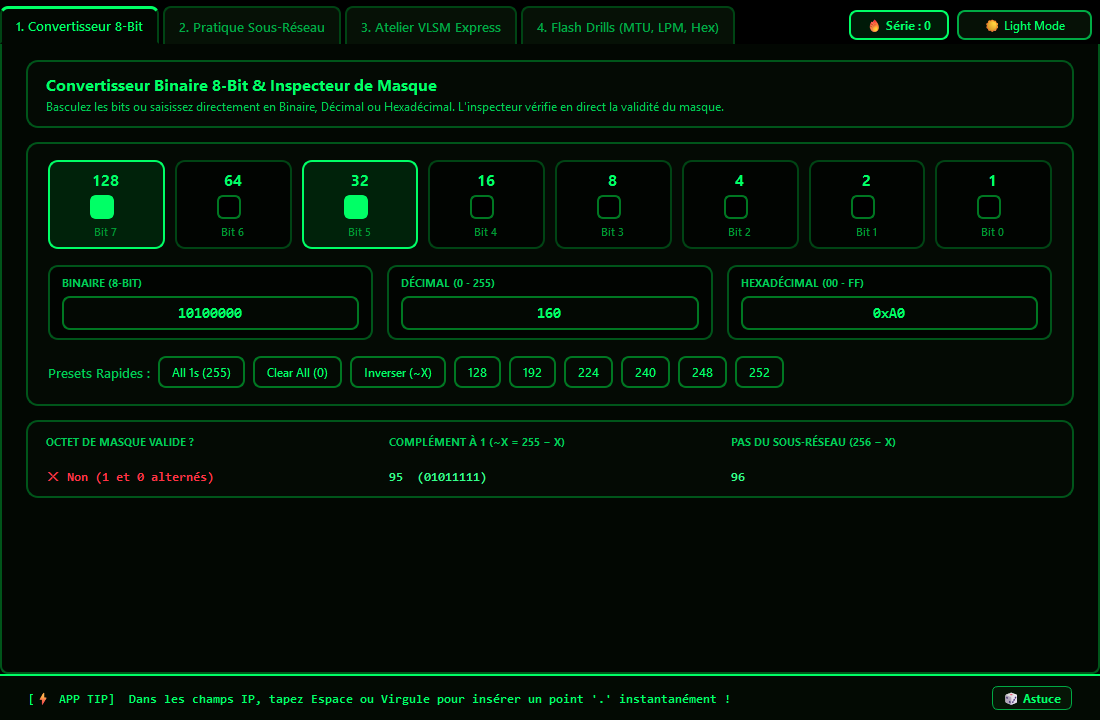
\includegraphics[width=0.88\textwidth]{../screenshots/02_tab1_mask_invalid_hacker.png}
    \caption{Onglet 1 en Mode Hacker Dark --- D\'etection en direct d'un octet de masque non contigu invalide (\texttt{160 = 10100000}$_2$).}
\end{figure}

\section{Impl\'ementation du Verrou Anti-R\'ecursion : \texttt{self.\_updating}}
Lorsqu'un utilisateur modifie le champ d\'ecimal, celui-ci d\'eclenche la mise \`a jour des cases \`a cocher et des champs binaire et hexad\'ecimal. Pour pr\'evenir une boucle d'\'ev\'enements infinie :
\begin{lstlisting}[language=Python]
def apply_value(self, val: int, source: str = ""):
    if self._updating:
        return
    self._updating = True
    try:
        val = max(0, min(255, val))
        self.current_value = val

        # 1. Mise a jour des 8 checkboxes sans declencher on_checkbox_toggled
        for i, cb in enumerate(self.bit_checkboxes):
            bit = (val >> (7 - i)) & 1
            cb.setChecked(bool(bit))

        # 2. Mise a jour des champs texte autres que la source active
        if source != "bin":
            self.bin_input.setText(f"{val:08b}")
        if source != "dec":
            self.dec_input.setText(str(val))
        if source != "hex":
            self.hex_input.setText(f"0x{val:02X}")

        # 3. Delegation a engine/ pour l'analyse pure
        analysis = IPv4MathEngine.analyze_octet(val)
        self.update_inspector_labels(analysis)
    finally:
        self._updating = False
\end{lstlisting}

\chapter{Onglet 2 : Pratique du Sous-R\'eseau \& Tiroir Binaire 32-bit (\texttt{ui/tab\_subnet.py})}

\section{Mod\`ele P\'edagogique \& Divulgation Progressive}
L'Onglet 2 (\texttt{SubnetPracticeTab}) est d\'edi\'e \`a l'entra\^inement intensif au calcul de sous-r\'eseaux IPv4 standard :
\begin{itemize}
    \item \textbf{Zone de Classification Rapide} : Choix de la classe (\texttt{A}, \texttt{B}, \texttt{C}) et de la port\'ee (\texttt{Publique}, \texttt{Priv\'ee RFC 1918}, \texttt{APIPA}, \texttt{Loopback}) avec feedback instantan\'e.
    \item \textbf{Tableau des 5 R\'eponses Cl\'es} : Network, First Host, Last Host, Broadcast, Next Subnet.
    \item \textbf{Tiroir Repliable 32 Bits} : D\'ecomposition bool\'eenne pas \`a pas (\texttt{IP ET Masque}, \texttt{Host ID Interne}, bits d'emprunt $b_S$ et bits d'h\^otes $b_H$).
\end{itemize}

\begin{figure}[!htbp]
    \centering
    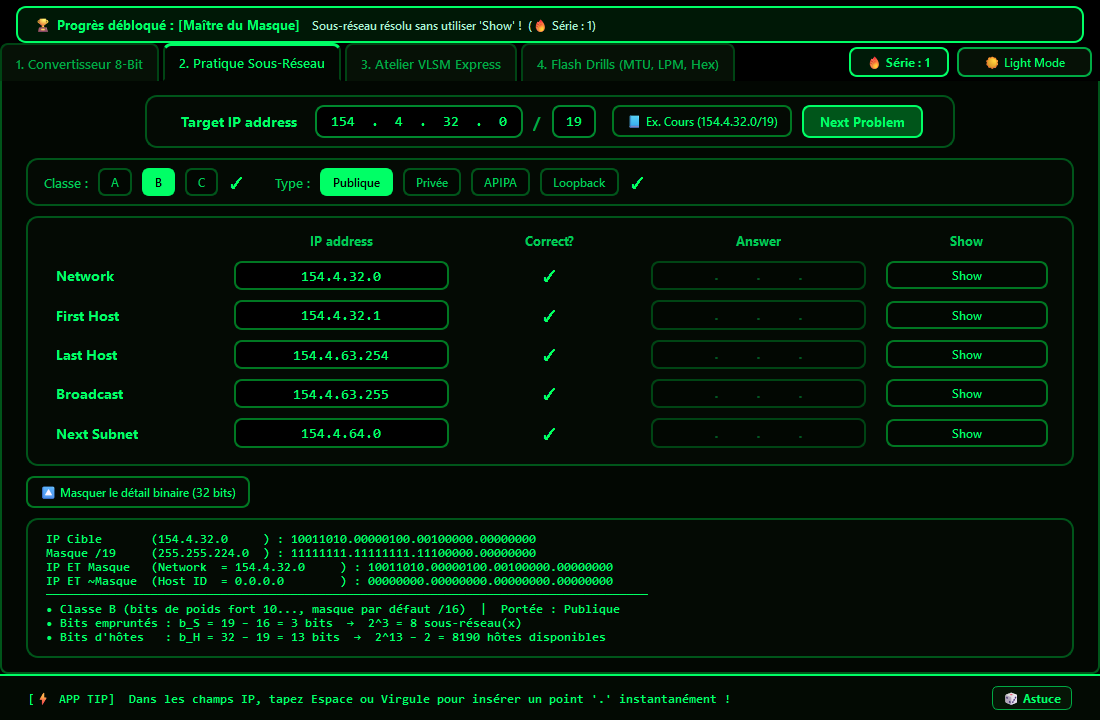
\includegraphics[width=0.88\textwidth]{../screenshots/04_tab2_subnet_hacker.png}
    \caption{Onglet 2 en Mode Hacker Dark --- R\'esolution de l'exercice avec d\'eploiement du tiroir binaire 32 bits.}
\end{figure}

\section{Gestion du Tiroir et Rafra\^ichissement QSS}
\begin{lstlisting}[language=Python]
def toggle_binary_drawer(self):
    """Bascule d'affichage du tiroir independamment de l'onglet actif."""
    should_show = self.drawer_card.isHidden()
    self.drawer_card.setVisible(should_show)
    self.btn_toggle_drawer.setText(
        "Masquer le detail binaire 32 bits" if should_show 
        else "Afficher le detail binaire 32 bits"
    )

def set_badge_state(self, badge: QLabel, solved: bool):
    """Application du pattern unpolish/polish pour reactualiser le style QSS."""
    badge.setProperty("solved", "true" if solved else "false")
    badge.style().unpolish(badge)
    badge.style().polish(badge)
\end{lstlisting}

\chapter{Onglet 3 : Atelier VLSM Express (\texttt{ui/tab\_vlsm.py})}

\section{Ergonomie "Z\'ero Surcharge Cognitive" \& Auto-Compl\'etion}
L'Atelier VLSM (\texttt{VlsmTab}) applique le principe : \textbf{l'\'etudiant prend les d\'ecisions d'architecture, l'outil s'occupe des d\'eductions m\'ecaniques}.
\begin{itemize}
    \item L'\'etudiant ordonne les besoins par ordre d\'ecroissant (\textit{Tri imp\'eratif}), d\'eduit le pr\'efixe optimal \texttt{/CIDR} ($2^h - 2 \ge N$), et calcule l'\textbf{Adresse R\'eseau}.
    \item D\`es que ces 3 champs sont corrects, le badge lat\'eral d'auto-compl\'etion s'allume en vert et renseigne imm\'ediatement la plage d'h\^otes utilisables (\texttt{.1} \`a \texttt{.126}), le broadcast et le masque.
\end{itemize}

\begin{figure}[!htbp]
    \centering
    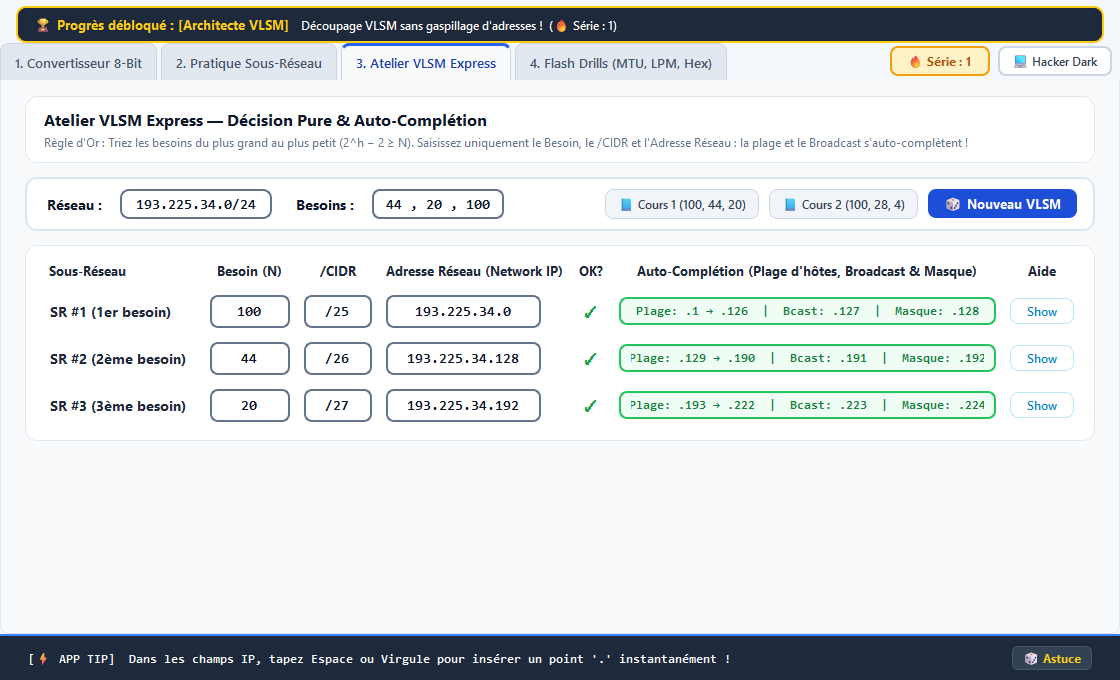
\includegraphics[width=0.88\textwidth]{../screenshots/05_tab3_vlsm_cours1_solved_light.png}
    \caption{Onglet 3 en Mode Modern Light --- Exercice Officiel du Cours 1 valid\'e avec auto-compl\'etion des badges.}
\end{figure}

\section{Changement d'Exercice sans Faux Positifs : \texttt{blockSignals(True)}}
Lorsqu'un nouveau preset est charg\'e (ex: Presets officiels du cours 1 et 2), les champs de saisie sont r\'einitialis\'es. Pour \'eviter que les signaux de texte modifi\'e ne d\'eclenchent intempestivement la validation :
\begin{lstlisting}[language=Python]
def load_problem(self, problem: VlsmProblem):
    self.current_problem = problem
    self.base_label.setText(f"Reseau Source : {problem.base_network_str}/{problem.base_cidr}")

    for row in self.rows:
        row.need_input.blockSignals(True)
        row.cidr_input.blockSignals(True)
        row.net_input.blockSignals(True)
        try:
            row.need_input.clear()
            row.cidr_input.clear()
            row.net_input.clear()
            row.summary_badge.setText("En attente de validation...")
            row.summary_badge.setProperty("solved", "false")
        finally:
            row.need_input.blockSignals(False)
            row.cidr_input.blockSignals(False)
            row.net_input.blockSignals(False)
\end{lstlisting}

\chapter{Onglet 4 : Flash Drills (\texttt{ui/tab\_drills.py})}

\section{Structure Multi-Exercices \`a Pagination \texttt{QStackedWidget}}
L'Onglet 4 (\texttt{DrillsTab}) regroupe trois sous-ateliers compl\'ementaires pilot\'es par un \texttt{QStackedWidget} :
\begin{enumerate}
    \item \textbf{Fragmentation MTU} : Calcul de la taille d'en-t\^ete ($\text{IHL} \times 4$), d\'ecoupage de la charge utile au multiple de 8 pr\`es, offset et indicateur MF.
    \item \textbf{Routage \& Longest Prefix Match (LPM)} : Analyse d'une table \`a 4 routes, d\'etermination de la route gagnante et identification de la r\`egle d\'ecisive (\textit{LPM}, \textit{Distance Administrative}, \textit{M\'etrique}, ou \textit{Route par D\'efaut}).
    \item \textbf{Checksum IPv4 (16 bits)} : Somme des 10 mots hexad\'ecimaux, retenue circulaire (\textit{end-around carry}) et compl\'ement \`a un final.
\end{enumerate}

\begin{figure}[!htbp]
    \centering
    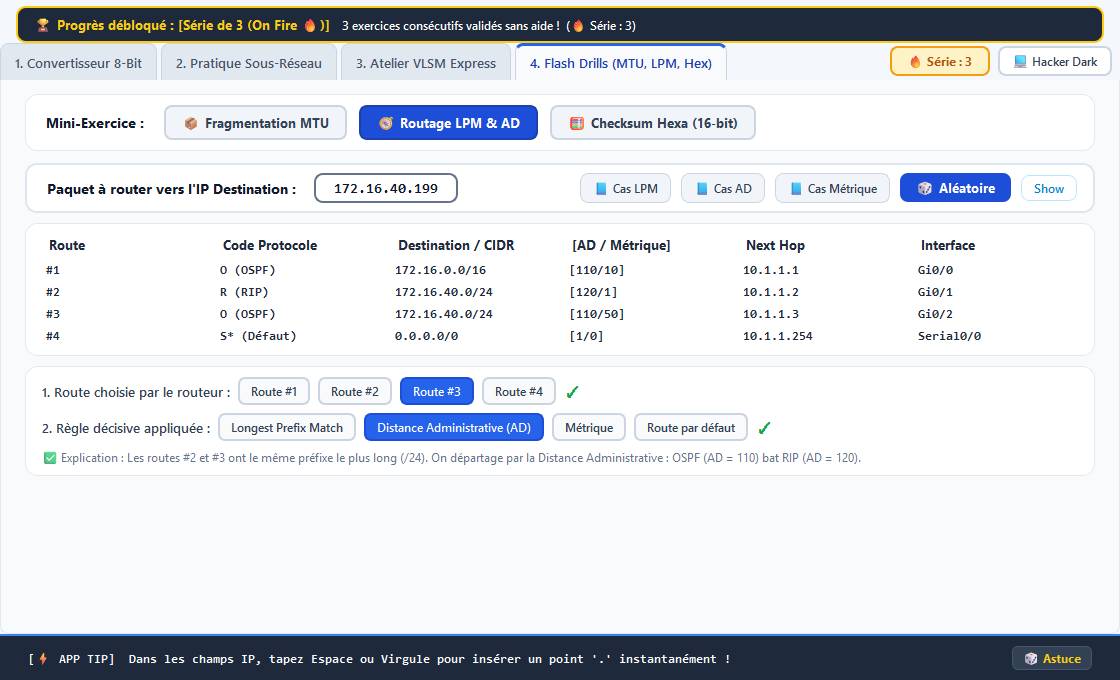
\includegraphics[width=0.88\textwidth]{../screenshots/08_tab4_drill_lpm_solved.png}
    \caption{Onglet 4 --- R\'esolution d'un exercice de routage LPM avec explications p\'edagogiques pas \`a pas.}
\end{figure}

\section{Algorithme de V\'erification LPM}
\begin{lstlisting}[language=Python]
def check_lpm_answer(self):
    selected_row = self.get_selected_route_row()
    selected_rule = self.combo_rule.currentText()
    problem = self.current_lpm_problem

    is_row_ok = (selected_row == problem.winning_row_id)
    is_rule_ok = (selected_rule == problem.decisive_rule)

    if is_row_ok and is_rule_ok:
        self.feedback_label.setText(f"Parfait ! {problem.explanation}")
        self.feedback_label.setProperty("status", "success")
        self.streak_mgr.record_win(without_show=not self.used_show, category="lpm_clean")
    else:
        self.feedback_label.setText("Incorrect. Verifiez la regle de priorite : LPM > AD > Metrique.")
        self.feedback_label.setProperty("status", "error")
\end{lstlisting}

% ============================================================================
% PARTIE VI : SYSTEME, PACKAGING & PORTAGE JAVA OOP
% ============================================================================
\part{Syst\`eme, Packaging \& Blueprint de Portage Java OOP}

\chapter{Cycle de Vie de l'Application \& Compilation Standalone}

\section{Point d'Entr\'ee \texttt{converter.py}}
Le cycle de vie d'une application PyQt6 s'articule en 4 \'etapes rigoureuses :
\begin{lstlisting}[language=Python]
import sys
from PyQt6.QtWidgets import QApplication
from ui.main_window import MainWindow

def main():
    app = QApplication(sys.argv)
    window = MainWindow()
    window.show()
    sys.exit(app.exec())

if __name__ == "__main__":
    main()
\end{lstlisting}
L'appel \texttt{app.exec()} d\'emarre la boucle d'\'ev\'enements principale et bloque jusqu'\`a la fermeture de la fen\^etre. \texttt{sys.exit()} relaie alors le code de sortie entier \`a l'OS.

\section{Compilation Binaire Standalone avec PyInstaller}
L'ex\'ecutable portable autonome (\texttt{converter.exe}, 38 Mo) est g\'en\'er\'e en encapsulant l'interpr\'eteur Python, PyQt6 et les scripts sans d\'ependance externe :
\begin{lstlisting}[language=bash]
pyinstaller --onefile --noconsole --name "converter" converter.py
\end{lstlisting}

\chapter{Blueprint de Portage vers Java 17/21 Orient\'e Objet}

\section{Correspondance des Mod\`eles de Donn\'ees (\texttt{record} Java)}
Toutes les structures \texttt{@dataclass(frozen=True)} de \texttt{engine/} se transposent sans aucune modification algorithmique en \texttt{record} Java :
\begin{lstlisting}[language=Java]
package ma.inpt.aseds.subnet.engine;

public record OctetAnalysis(
    int value,
    String binaryStr,
    String hexStr,
    boolean isValidMaskOctet,
    int onesComplement,
    String onesComplementBinary,
    int blockSize
) {}
\end{lstlisting}

\section{Pi\`eges de l'Arithm\'etique 32 bits en Java (\texttt{int} sign\'e vs \texttt{long})}
En Java, le type primitif \texttt{int} est sign\'e sur 32 bits (de $-2^{31}$ \`a $2^{31}-1$). Ainsi, \texttt{0xFFFFFFFF} vaut $-1$.
\begin{enumerate}
    \item Utiliser le type \textbf{\texttt{long} (64 bits)} ou l'op\'erateur de d\'ecalage logique non sign\'e \textbf{\texttt{>>>}} pour les adresses 32 bits :
\begin{lstlisting}[language=Java]
long maskInt = (cidr > 0) ? ((0xFFFFFFFFL << (32 - cidr)) & 0xFFFFFFFFL) : 0L;
long wildcardInt = (~maskInt) & 0xFFFFFFFFL;
long networkInt = ipInt & maskInt;
long hostIdInt = ipInt & wildcardInt;
long broadcastInt = networkInt | wildcardInt;
\end{lstlisting}
    \item Pour le Checksum 16 bits :
\begin{lstlisting}[language=Java]
int carried = rawSum;
while (carried > 0xFFFF) {
    carried = (carried & 0xFFFF) + (carried >>> 16);
}
int checksum = (~carried) & 0xFFFF;
\end{lstlisting}
\end{enumerate}

\section{Architecture de Packages Java Recommand\'ee}
\begin{itemize}
    \item \texttt{ma.inpt.aseds.subnet.engine} : 100\,\% Java standard, couvert par des tests unitaires \textbf{JUnit 5}.
    \item \texttt{ma.inpt.aseds.subnet.ui} : Vues d'interface d\'evelopp\'ees en JavaFX 21 ou Swing FlatLaf reprenant les m\^emes feuilles de style CSS/QSS.
\end{itemize}

\chapter*{Conclusion \& Synth\`ese P\'edagogique}
\addcontentsline{toc}{chapter}{Conclusion \& Synth\`ese P\'edagogique}
Le pr\'esent manuel compile et formalise l'int\'egralit\'e des connaissances p\'edagogiques et d'ing\'enierie logicielle int\'egr\'ees dans la suite d'apprentissage \textbf{IPv4 Subnet Toolkit v1.2.0}. 

En combinant une compr\'ehension math\'ematique rigoureuse de l'alg\`ebre binaire IPv4, le respect strict de la Clean Architecture et des principes d'ergonomie cognitive modernes, ce projet constitue une r\'ef\'erence compl\`ete pour les \'etudiants et ing\'enieurs de l'INPT dans leur ma\^itrise des r\'eseaux informatiques et de la conception logicielle robuste.

\end{document}
